
%!TEX root = ../template.tex
%%%%%%%%%%%%%%%%%%%%%%%%%%%%%%%%%%%%%%%%%%%%%%%%%%%%%%%%%%%%%%%%%%%%
%% chapter8.tex
%% NOVA thesis document file
%%
%% Chapter with lots of dummy text
%%%%%%%%%%%%%%%%%%%%%%%%%%%%%%%%%%%%%%%%%%%%%%%%%%%%%%%%%%%%%%%%%%%%

\typeout{NT FILE chapter8.tex}%

\chapter{Results and Validation}
\label{cha:results}

The previous chapters introduced the methods developed for this thesis. A few examples were presented to help follow the explanation and description of the methods. In this chapter, we go further into testing the algorithms in corresponding tasks on the datasets introduced in Chapter \ref{cha:dataset}. The methods are tested and validated to provide evidence that the work developed in this thesis is relevant and contributes to the state of the art he time series data mining field.
\par
Considering the diversity of methods developed, this chapter will be divided into every single contribution, providing results for each one of them. We will start with the methods developed under the topics of Chapter \ref{cha:segmentation}, more specifically for time series segmentation.

\section{Segmentation}

\subsection{Novelty Segmentation}

In this section, we present several examples of how the \textit{nova} function, retrieved from the \gls{ssm}, is useful for the segmentation of time series. The reader will appreciate that we also provide a measure of the algorithm's performance considering ground truth events from public benchmarks, while also comparing our proposed solution with state-of-the-art methods for change point detection from the \textit{Turing Change Point Detection Benchmark} \cite{cpd_alan}.
\par
This section is divided into three main categories: (1) Validation in segmentation datasets, (2) comparison with state-of-the-art art methods, and (3) discussion of the results obtained.

\subsubsection{Performance on Public Datasets}

The datasets that were used to test and validate this method have categorized labels that were used to generate ground-truth events. These include different contexts (\gls{har}, Hand Posture, Noise Detection, etc...) and different types of data (Inertial data, \gls{emg} and \gls{ecg}).
\par
The method has been computed in the same conditions and by following the same procedure for all records of all datasets. The features used have been the same for each record, varying the time scale parameter, the overlap size of the sliding window, and the kernel size. The peak detection strategy was the same for all records, which is based on a threshold mechanism. The threshold value varied for each record. Results for publicly available datasets are presented in Tables \ref{tab:overall_cpd} and \ref{tab:overall_cpd_dist}. Table \ref{tab:overall_cpd} indicates the performance in detecting the change point events. Overall results for each time series of each dataset can be checked in Appendix \ref{app:tables_detailed}

\begin{table*}
	\begin{center}
		\begin{tabular}{lccccccccc}
			\toprule
			Dataset & Signals & \# Ch & Task & TP & FP & FN & Prec (\%) & Rec (\%) & F1 (\%) \\
			\toprule
			Dataset 1 & ACC & 3 & HACP & 98 & 16 & 16 & 0.860 & 0.860 & 0.860 \\
			Dataset 2 & ACC-GYR & 6 & HACP & 157 & 18 & 22 & 0.897 & 0.877 & 0.887 \\
			Dataset 3 & ACC-GYR & 6 & HACP & 1378 & 313 & 263 & 0.815 & 0.840 & 0.827 \\
			Dataset 4 & ACC-GYR & 12 & HACP & 499 & 71 & 38 & 0.875 & 0.929 & 0.902 \\
			Dataset 5 & \gls{emg} & 8 & Act/Rel & 309 & 0 & 0 & 1.000 & 1.000 & 1.000 \\
			Dataset 6  & \gls{ecg} & 1 & Noise & 132 & 25 & 10 & 0.841 & 0.930 & 0.883 \\
			Dataset 7  & \gls{ecg} & 4 & Noise & 21 & 2 & 3 & 0.913 & 0.875 & 0.894 \\
			\midrule
			Total & N.A. & N.A. & N.A. & 2629 & 465 & 352 & 0.850 & 0.882 & 0.866 \\
			\bottomrule
		\end{tabular}
	\end{center}
	\caption{Overall results for the performance of the method on novelty segmentation. The dimension of the records is presented on the column \textit{\# Ch}, as well as the types of signals used and the task in which  applied (HACP - Human Activity Segmentation; Act/Rel - Activation/Relaxation of the \gls{emg} and Noise detection). The overall measures of Recall and Precision were micro-averaged.}
	\label{tab:overall_cpd}
\end{table*}


\begin{table}
	\begin{center}
        \begin{tabular}{lccc}
            \toprule
			Dataset & $T_s$ (s) & $MAE/T_s$ & $MsE/T_s$ \\
			\toprule
			Dataset 1 & 5 & 0.53 & -0.12 \\
			Dataset 2 & 10 & 0.29 & -0.07 \\
			Dataset 3 & 1 & 0.34 & -0.04 \\
			Dataset 4 & 25 & 0.23 & -0.00 \\
			Dataset 5 & 1 & 1 & -0.13 \\
			Dataset 6 & 10 & 0.12 & -0.09 \\
			Dataset 7 & 1 & 0.17 & -0.06 \\
			\midrule
			Average & N.A. & 0.32 & -0.07 \\
			\bottomrule
		\end{tabular}
	\end{center}
	\caption{Distance error as a ratio of the time scale ($T_s$) for the detected TP.}
	\label{tab:overall_cpd_dist}
\end{table}

The results and the examples provided in the previous Chapter show that the proposed method has a good performance in detecting events, in real, complex, multivariate, and diverse datasets. The results are consistent, supporting that the proposed method is reliable to use in multiple types of data and different contexts.
\par
The method achieved an overall macro-averaged 85.0\% of Precision, 87.2\% of Recall, and an F1 measure of 86.1\%. Individually, the worst performance was found on Dataset 3, although all the Datasets accounted for similar results. A more comprehensive discussion on \textit{FN} and \textit{FP} will be presented in a further section. More details are also provided regarding the time discrepancies between ground truth and estimated events.

\subsubsection{Comparison with SOA Methods}

In order to compare the proposed method with state of the art approaches, we used a benchmark provided by the Alan Turing Institute \cite{cpd_alan}. The performance was evaluated by computing the proposed method to search for change point events in each of the time series available. The time scale and threshold values for peak detection were selected empirically and available in Table \ref{tab:app_ati_parameters}. The results are summarized in Table \ref{tab:alanturing} and Figure \ref{fig:cdd_alant}. Both cases show the F1 score. The performance considered for other methods was selected as the best score of each method available on the benchmark \cite{cpd_alan}.

\begin{table*}[h!]
\begin{adjustbox}{width=\textwidth}
    \begin{tabular}{l|c|cccccccccccccc}
    Dataset & \textsc{Nova} & \textsc{amoc} & \textsc{binseg} & \textsc{bocpd} & \textsc{bocpdms} & \textsc{cpnp} & \textsc{ecp} & \textsc{kcpa} & \textsc{pelt} & \textsc{prophet} & \textsc{rbocpdms} & \textsc{rfpop} & \textsc{segneigh} & \textsc{wbs} & \textsc{zero}\\
    \hline
    \cellcolor{gray!100}\verb+bank+ & \cellcolor{gray!100}0 & \cellcolor{gray!100}\textbf{1.000} & \cellcolor{gray!100}\textbf{1.000} & \cellcolor{gray!100}\textbf{1.000} & \cellcolor{gray!100}0.500 & \cellcolor{gray!100}0.054 & \cellcolor{gray!100}0.200 & \cellcolor{gray!100}0.333 & \cellcolor{gray!100}0.400 & \cellcolor{gray!100}\textbf{1.000} & \cellcolor{gray!100}T & \cellcolor{gray!100}0.015 & \cellcolor{gray!100}\textbf{1.000} & \cellcolor{gray!100}0.043 & \cellcolor{gray!100}\textbf{1.000}\\
    \verb+bitcoin+ & \cellcolor{SeaGreen!04}\textbf{0.694} & 0.507 & 0.690 & 0.733 & 0.533 & 0.611 & 0.625 & 0.665 & 0.735 & 0.446 & T & 0.284 & 0.735 & 0.690 & 0.450\\
    \verb+brent_spot+ & \cellcolor{blue!20}\textbf{0.861} & 0.465 & 0.670 & 0.609 & 0.239 & 0.607 & 0.636 & 0.553 & 0.586 & 0.249 & T & 0.521 & 0.586 & 0.564 & 0.315\\
    \verb+businv+ & \cellcolor{blue!40}\textbf{0.927} & 0.588 & 0.588 & 0.588 & 0.455 & 0.386 & 0.370 & 0.294 & 0.490 & 0.275 & 0.370 & 0.261 & 0.588 & 0.289 & 0.588\\
    \verb+centralia+ & \cellcolor{SeaGreen!01}0.984 & 0.909 & \textbf{1.000} & \textbf{1.000} & \textbf{1.000} & \textbf{1.000} & 0.909 & \textbf{1.000} & \textbf{1.000} & 0.763 & 0.846 & \textbf{1.000} & \textbf{1.000} & 0.556 & 0.763\\
    \verb+children_per_woman+ & \cellcolor{blue!16}\textbf{0.879} & 0.678 & 0.663 & 0.712 & 0.405 & 0.344 & 0.551 & 0.525 & 0.637 & 0.310 & 0.504 & 0.246 & 0.637 & 0.500 & 0.507\\
    
    \verb+co2_canada+ & \cellcolor{SeaGreen!07}0.851 & 0.544 & 0.856 & \textbf{0.924} & 0.479 & 0.642 & 0.875 & 0.867 & 0.670 & 0.482 & 0.542 & 0.569 & 0.872 & 0.681 & 0.361\\
    
    \verb+construction+ & \cellcolor{blue!23}0.933 & 0.696 & 0.709 & 0.709 & 0.410 & 0.602 & 0.709 & 0.634 & 0.709 & 0.324 & 0.340 & 0.185 & 0.709 & 0.523 & 0.696\\
    
    \verb+debt_ireland+ & \cellcolor{SeaGreen!01}0.974 & 0.760 & \textbf{1.000} & \textbf{1.000} & 0.892 & 0.958 & 0.980 & \textbf{1.000} & \textbf{1.000} & 0.469 & 0.748 & 0.824 & \textbf{1.000} & 0.538 & 0.469\\
    
    \verb+gdp_argentina+ & \cellcolor{SeaGreen!02}\textbf{0.968} & 0.889 & 0.947 & 0.947 & 0.583 & 0.818 & 0.889 & 0.800 & 0.947 & 0.615 & 0.452 & 0.615 & 0.947 & 0.421 & 0.824\\
    
    \verb+gdp_croatia+ & \textbf{1.000} & \textbf{1.000} & 0.824 & \textbf{1.000} & 0.583 & \textbf{1.000} & 0.824 & 0.583 & 0.824 & 0.824 & 0.824 & 0.400 & 0.824 & 0.167 & 0.824\\
    
    \verb+gdp_iran+ & \cellcolor{SeaGreen!06}0.921 & 0.696 & 0.652 & 0.862 & 0.492 & 0.620 & 0.824 & 0.734 & 0.808 & 0.652 & 0.737 & 0.636 & 0.808 & 0.576 & 0.652\\
    
    \verb+gdp_japan+ & \textbf{1.000} & \textbf{1.000} & 0.889 & \textbf{1.000} & 0.615 & 0.667 & \textbf{1.000} & 0.500 & 0.889 & 0.889 & 0.889 & 0.222 & 0.889 & 0.222 & 0.889\\
    
    \verb+global_co2+ & \cellcolor{SeaGreen!30}0.625 & 0.929 & 0.929 & 0.889 & 0.458 & 0.667 & \textbf{0.929} & 0.667 & 0.929 & 0.463 & 0.547 & 0.293 & 0.929 & 0.250 & 0.846\\
    
    \verb+homeruns+ & \cellcolor{blue!10}\textbf{0.933} & 0.812 & 0.829 & 0.829 & 0.650 & 0.650 & 0.829 & 0.829 & 0.812 & 0.723 & 0.397 & 0.661 & 0.812 & 0.664 & 0.659\\
    
    \verb+iceland_tourism+ & \cellcolor{SeaGreen!40}0.652 & 0.947 & 0.947 & 0.947 & 0.486 & 0.391 & \textbf{1.000} & 0.486 & 0.643 & 0.220 & 0.667 & 0.200 & 0.947 & 0.200 & 0.947\\
    
    \verb+jfk_passengers+ & \cellcolor{blue!20}\textbf{0.978} & 0.776 & 0.776 & 0.776 & 0.650 & 0.602 & 0.651 & 0.437 & 0.776 & 0.354 & T & 0.491 & 0.776 & 0.437 & 0.723\\
    
    \verb+lga_passengers+ & \cellcolor{SeaGreen!01}0.885 & 0.561 & 0.620 & 0.704 & 0.563 & 0.606 & \textbf{0.892} & 0.526 & 0.537 & 0.366 & T & 0.592 & 0.537 & 0.674 & 0.535\\
    
    \cellcolor{gray!100}\verb+measles+ & \cellcolor{gray!100}0 & \cellcolor{gray!100}\textbf{0.947} & \cellcolor{gray!100}\textbf{0.947} & \cellcolor{gray!100}\textbf{0.947} & \cellcolor{gray!100}0.486 & \cellcolor{gray!100}0.118 & \cellcolor{gray!100}0.080 & \cellcolor{gray!100}0.281 & \cellcolor{gray!100}0.153 & \cellcolor{gray!100}0.391 & \cellcolor{gray!100}F/T & \cellcolor{gray!100}0.030 & \cellcolor{gray!100}\textbf{0.947} & \cellcolor{gray!100}0.041 & \cellcolor{gray!100}\textbf{0.947}\\
    
    \verb+nile+ & \textbf{1.000} & \textbf{1.000} & \textbf{1.000} & \textbf{1.000} & 0.800 & \textbf{1.000} & \textbf{1.000} & 0.824 & \textbf{1.000} & 0.824 & 0.667 & \textbf{1.000} & \textbf{1.000} & \textbf{1.000} & 0.824\\
    
    \verb+ozone+ & \cellcolor{SeaGreen!0}0.857 & 0.776 & 0.723 & 0.857 & 0.778 & 0.750 & \textbf{1.000} & 0.667 & \textbf{1.000} & 0.723 & 0.651 & 0.429 & \textbf{1.000} & 0.286 & 0.723\\
    
    \verb+quality_control_1+ & \textbf{1.000} & \textbf{1.000} & \textbf{1.000} & \textbf{1.000} & 0.667 & 0.667 & \textbf{1.000} & 0.667 & \textbf{1.000} & 0.500 & 0.286 & 0.667 & \textbf{1.000} & 0.667 & 0.667\\
    
    \verb+quality_control_2+ & \textbf{1.000} & \textbf{1.000} & \textbf{1.000} & \textbf{1.000} & 0.667 & \textbf{1.000} & \textbf{1.000} & \textbf{1.000} & \textbf{1.000} & 0.750 & .429 & \textbf{1.000} & \textbf{1.000} & \textbf{1.000} & 0.750\\
    
    \verb+quality_control_3+ & \textbf{1.000} & \textbf{1.000} & \textbf{1.000} & \textbf{1.000} & 0.766 & 0.571 & \textbf{1.000} & \textbf{1.000} & \textbf{1.000} & 0.667 & T & 0.800 & \textbf{1.000} & \textbf{1.000} & 0.667\\
    
    \verb+quality_control_4+ & \cellcolor{blue!10}0.974 & 0.810 & 0.873 & 0.787 & 0.561 & 0.658 & 0.726 & 0.658 & 0.780 & 0.780 & T & 0.241 & 0.780 & 0.608 & 0.780\\
    
    \cellcolor{gray!100}\verb+quality_control_5+ & \cellcolor{gray!100}0 & \cellcolor{gray!100}\textbf{1.000} & \cellcolor{gray!100}\textbf{1.000} & \cellcolor{gray!100}\textbf{1.000} & \cellcolor{gray!100}0.500 & \cellcolor{gray!100}\textbf{1.000} & \cellcolor{gray!100}\textbf{1.000} & \cellcolor{gray!100}\textbf{1.000} & \cellcolor{gray!100}\textbf{1.000} & \cellcolor{gray!100}\textbf{1.000} & \cellcolor{gray!100}0.500 & \cellcolor{gray!100}\textbf{1.000} & \cellcolor{gray!100}\textbf{1.000} & \cellcolor{gray!100}\textbf{1.000} & \cellcolor{gray!100}\textbf{1.000}\\
    
    \verb+rail_lines+ & \cellcolor{SeaGreen!06}\textbf{0.909} & 0.846 & 0.846 & 0.966 & 0.889 & 0.966 & {0.966} & 0.800 & 0.846 & 0.537 & 0.730 & 0.615 & 0.889 & 0.205 & 0.537\\
    
    \verb+ratner_stock+ & \cellcolor{blue!07}0.933 & 0.776 & 0.824 & 0.868 & 0.559 & 0.396 & 0.776 & 0.754 & 0.824 & 0.280 & T & 0.203 & 0.824 & 0.378 & 0.571\\
    
    \verb+robocalls+ & \cellcolor{blue!01}0.979 & 0.800 & 0.966 & 0.966 & 0.750 & 0.862 & 0.966 & 0.966 & 0.966 & 0.636 & 0.846 & 0.714 & 0.966 & 0.714 & 0.636\\
    
    \verb+scanline_126007+ & \cellcolor{SeaGreen!04}0.887 & 0.710 & 0.920 & \textbf{0.921} & 0.829 & 0.906 & 0.870 & 0.838 & 0.889 & 0.644 & T & 0.649 & 0.889 & 0.818 & 0.644\\
    
    \verb+scanline_42049+ & \cellcolor{blue!01}\textbf{0.977} & 0.485 & 0.879 & 0.962 & 0.889 & 0.713 & 0.910 & 0.908 & 0.910 & 0.269 & T & 0.460 & 0.910 & 0.650 & 0.276\\
    
    \verb+seatbelts+ & \cellcolor{SeaGreen!20}0.659 & 0.824 & \textbf{0.838} & 0.683 & 0.583 & 0.735 & 0.683 & 0.621 & 0.683 & 0.452 & 0.383 & 0.563 & 0.735 & 0.583 & 0.621\\
    
    \verb+shanghai_license+ & \cellcolor{blue!01}\textbf{0.979} & 0.966 & 0.868 & 0.868 & 0.605 & 0.600 & 0.868 & 0.465 & 0.868 & 0.532 & 0.389 & 0.357 & 0.868 & 0.385 & 0.636\\
    
    \cellcolor{gray!100}\verb+uk_coal_employ+ & \cellcolor{gray!100}F & \cellcolor{gray!100}F & \cellcolor{gray!100}F & \cellcolor{gray!100}F & \cellcolor{gray!100}0.617 & \cellcolor{gray!100}F & \cellcolor{gray!100}0.513 & \cellcolor{gray!100}0.513 & \cellcolor{gray!100}F & \cellcolor{gray!100}\textbf{0.639} & \cellcolor{gray!100}F & \cellcolor{gray!100}F & \cellcolor{gray!100}F & \cellcolor{gray!100}F & \cellcolor{gray!100}0.513\\
    
    \verb+unemployment_nl+ & \cellcolor{SeaGreen!07}0.820 & 0.742 & \textbf{0.889} & 0.876 & 0.592 & 0.747 & 0.755 & 0.744 & 0.788 & 0.566 & F/T & 0.628 & 0.788 & 0.801 & 0.566\\
    
    \verb+us_population+ & \cellcolor{SeaGreen!40}0.636 & \textbf{1.000} & 0.889 & \textbf{1.000} & 0.615 & 0.232 & 0.471 & 0.276 & 0.500 & 0.159 & T & 0.889 & 0.889 & 0.113 & 0.889\\
    
    \verb+usd_isk+ & \cellcolor{blue!20}0.914 & 0.785 & 0.704 & 0.785 & 0.678 & 0.674 & 0.785 & 0.601 & 0.657 & 0.489 & 0.510 & 0.462 & 0.678 & 0.636 & 0.489\\
    
    \verb+well_log+ & \cellcolor{SeaGreen!10}0.814 & 0.336 & 0.914 & 0.832 & 0.743 & 0.822 & \textbf{0.928} & 0.776 & 0.873 & 0.149 & T & 0.923 & 0.873 & 0.832 & 0.237\\
    
    \hline
    
    \verb+apple+ & \cellcolor{blue!03}\textbf{0.949} &  &  & 0.916 & 0.445 &  & 0.745 & 0.634 &  &  & F/T &  &  &  & 0.594\\
    
    \verb+bee_waggle_6+ & \cellcolor{SeaGreen!28}0.657 &  &  & \textbf{0.929} & 0.481 &  & 0.233 & 0.634 &  &  & 0.245 &  &  &  & \textbf{0.929}\\
    
    \verb+occupancy+ & \cellcolor{blue!02}0.953 &  &  & 0.919 & 0.735 &  & \textbf{0.932} & 0.812 &  &  & F/T &  &  &  & 0.341\\
    
    \verb+run_log+ & 0.994 &  &  & \textbf{1.000} & 0.469 &  & 0.990 & 0.909 &  &  & 0.380 &  &  &  & 0.446\\
    
    \bottomrule
    
    \textbf{Average F1-measure (1D)} & \cellcolor{blue!05}\textbf{0.845} & 0.739 & 0.798 & 0.822 & 0.596 & 0.651 & 0.784 & 0.657 & 0.766 & 0.482 & 0.354 & 0.517 & 0.797 & 0.517 & 0.599\\
    
    \bottomrule
    
    \textbf{Average F1-measure (ALL)} & \cellcolor{blue!05}\textbf{0.871} & n.a. & n.a. & 0.855 & 0.604 & n.a. & 0.797 & 0.683 & n.a. & n.a. & 0.343 & n.a. & n.a. & n.a. & 0.61
    \end{tabular}
\end{adjustbox}
    \caption{Comparison of performance between the proposed method (\textit{Nova}) and other algorithms. The colors indicate if the other algorithms were better (Green) or worse (Blue) in performance than the \textit{Nova} method for a specific dataset. Time series from \textit{apple}, \textit{bee\_waggle\_6}, \textit{occupancy} and \textit{run\_log} are multivariate. The average results are grouped on the last row. Averages did not considered the gray columns, since these would imply that no change point should be detected, or an error on the signal was present. \textit{T} appears when the method timedout, \textit{M} and \textit{F} when the method failed in compiling}.
    \label{tab:alanturing}
\end{table*}

As presented in Figure \ref{fig:cdd_alant}, the critical distance diagram ranks the proposed method in the top four, without a significant difference in performance (considering methods that only work in uni-dimensional datasets). The average F1 measure is 79.6\% for both uni and multi-dimensional datasets. Two of the F1 measures are null because, in these two time series, no change point was supposed to be found, but the proposed method is not yet prepared to return no results. 
\par
The results obtained in this benchmark demonstrate that this method is promising, having a performance that competes with several state-of-the-art methods in the problem of novelty segmentation. We highlight that the proposed method applies to multi-dimensional time series, while two of the best ranked methods in Figure \ref{fig:cdd_alant} are not. In addition, this method is not solely focused on retrieving segmentation points, but also provides additional layers of information, namely periodic changes and the level of similarity between segments, which is an advantage over the \textit{BOCPD}.

\begin{figure}
    \centering
    \includegraphics[width=\linewidth]{critical_distance_novelty.pdf}
    \caption{Critical distance diagram comparing the methods used in \cite{cpd_alan} (except \textit{RBOCPDMS}) and the \textit{novelty function} (\textit{nova} - highlighted in SeaGreen). The performance measure corresponds to the F1-score for all single-dimension datasets of the benchmark (except the ones highlighted in gray in Figure \ref{tab:alanturing}).}
    \label{fig:cdd_alant}
\end{figure}

\subsubsection{Insights on FN and FP}

In this section, we present a more comprehensive discussion regarding the \textit{FN} and \textit{FP} counts. Regarding \textit{FP} counts, these were found in several datasets to be mostly associated with changes on the signal that were not labeled. Since our proposed approach is \textit{unsupervised}, most changes that appear significant will be detected, even if not explicitly labeled. This is visible, for example, in Figure \ref{fig:use_case1}, where the subject was climbing stairs but something happened during the acquisition that makes the signal change dramatically. We found the same type of mislabeled data on Datasets 2, 3, and 4, with Dataset 3 having the worst rate of \textit{FP}. Specifically, in this case, part of these \textit{FP} were due to subsequences that were not annotated, for instance, in Figure \ref{fig:har1_dataset} we highlighted in light yellow areas where something happened but no label is given. As most of these datasets were used for classification purposes, some labels were not given, but our method, being unsupervised and not focused on classification tasks, can find these occurrences. The method also has a worse rate of \textit{FN} for this dataset. We can explain these by the difficulty of the method in finding the labeled transitions between static positions (sit-to-stand, stand-to-sit, stand-to-laying, etc...). The method was able to find these as one segment but was not able to find the start and end of each of these transitions, as it was labeled. Detecting the start and end of these would require smaller window sizes.
\par
For datasets with categorized events, which are a transition between one categorized \textit{subsequence} to another, we can evaluate from which categories the events were missed. Then, identify if specific types of events were the cause of the \textit{FN} count rate. Figure \ref{fig:fn_dataset2} indicates the F1-score of the \textit{nova} function in detecting the different transition categories of events using the color and size of circles associated with each event category. The activities before and after change point events are sorted in columns. Each row is associated with a specific event category and corresponding circle, which color indicates the detection's accuracy, while the size indicates the percentage of events associated with the corresponding event category.

%\begin{wrapfigure}{r}{0.5\linewidth}
%    \centering
%    \includegraphics[width=\linewidth]{FN_example.pdf}
%    \caption{F1-score in detecting each of the categories of event transition from Dataset 2. \textbf{Pre CP} - activity performed before the change point event; \textbf{Pos CP} - activity performed after the change point. The performance in detecting each transition is showed by the circles color.}
%    \label{fig:fn_dataset2}
%\end{wrapfigure}

As the results illustrated in Figure \ref{fig:fn_dataset2}, the F1-score is lower in cases of activities with similar characteristics on time series. In this case, the transition between $Walking \xrightarrow[]{} Walking Upstairs$ has the lowest accuracy rate. However, transitions between $Walking \xrightarrow[]{} Walking up/downstairs$, as well as transitions between $Sitting \xrightarrow[]{} Standing$, are more difficult to detect. These results are supported by Figure \ref{fig:fn_dataset2}, where peaks in the \textit{nova} function are smaller for these transitions. Although a significant portion of these events have been missed, the problem is not necessarily that the \gls{ssm} has not the checkerboard pattern. In these cases, these more subtle changes were overshadowed by very significant changes, such as $Walking \xrightarrow[]{} Standing$. Nevertheless, a re-normalization of the \gls{ssm} segment of interest can help better visualize the differences that were initially hidden. 
\par
An example of the enhancement process is better seen on Figure \ref{fig:example1_zoom} from Chapter \ref{cha:segmentation}. The block $A$ is highlighted, showing clearly the three modes of the time series. Now that we only focus on that segment, we can perceive these transitions. This example demonstrates that this tool has the potential of enhancing the detection of several transitions in a hierarchical process by re-normalizing segments of an initial segmentation. This would come without a significant extra computational cost since these measures of the \gls{ssm} are already computed. Nevertheless, there is the potential of finding extra undesired events depending on the threshold level.

\subsubsection{Comparisons to Related Work}

We will now look for specific datasets from the \textit{TCPD} benchmark that should be highlighted considering the results obtained. In Table \ref{tab:alanturing}, we notice that datasets, such as \textit{global\_co2}, \textit{iceland\_tourism}, \textit{lga\_passenger} and \textit{us\_population}, have a lower score when compared to the best methods. In the other end, the proposed method was better than the best methods in datasets \textit{bitcoin}, \textit{brent\_spot}, \textit{busivn} and \textit{jfk\_passenger}. From these results, we notice that the proposed method is more fragile when events occur as a slight change in the trend of a signal, such as the case of \textit{global\_co2} or \textit{us\_population} records, while it is better for more significant changes in a pattern, amplitude or other property.
\par
The results show that this method is highly competitive in performing event detection in time series, with high performance scores in real-world datasets. From all methods tested in the \textit{TCPD benchmark}, only the \textit{BOCPD} method was able to obtain similar results (Figure \ref{fig:cdd_alant} and Table \ref{tab:alanturing}), considering also multidimensional datasets, but it does so with an optimization of many parameters. The proposed method is being computed with several parameters as well but has the potential to accept only one.
\par
One of the other great advantages of the proposed method is that it also provides rich visual feedback, which can be perfect to support the analyst in interpreting a time series. The content of the \gls{ssm} goes beyond change point detection, providing relevant information about periodicity and similarity.

\subsubsection{Effects of Window Size and Overlap}

Several parameters affect the ability to detect the desired patterns. These are the window size, the overlap percentage, and the kernel size. Although in this work we used all three parameters, these can potentially be combined into a single one. We only considered entry parameters on the method that affect the visual output and novelty function. We do not consider the parameters for the threshold-based peak strategy used.
\par
These parameters can be explained with the analogy of a camera. The window size works like the \textit{zoom function}, defining the scale of interest in the time series. Larger windows correspond to lower \textit{zoom values} and will compute the similarity of larger \textit{subsequences}, while smaller windows are like a \textit{zoom-in} function on the time series, searching for any small detail that might be a change. The overlap percentage is the \textit{camera sensor}, which defines the pixel resolution of the image and works as a downsampler of the time series. A full resolution of the \gls{ssm} is only achieved with total overlap, and the lower the overlap percentage, the less accurate are the highlighted changes.
\par
These two parameters are fundamental for the success of the event detection process. This is most evident in some of the datasets where we applied the proposed method, since the larger the time scale used, the larger the \gls{mae} in the detected events. For instance, in \textit{Dataset 4}, the time series are very large (3 minutes for each of the 18 activities, at 20 Hz), which due to computation time and memory allocation constraints, we used a larger time window with a lower overlap percentage. The result was an increase in the \gls{mae}. Still, this error was also affected by delays in the ground truth, as explained in the previous section.
\par
On the other hand, the sliding kernel computes the sharpness of the changes detected with the novelty function. The larger it is, the smoother will be the resulting function. Potentially, even with a small decrease in accuracy, the kernel size could be calculated as a ratio of the window size. The overlap percentage should be maximized and based on the memory available to perform the \gls{ssm} computation. With this, we could define the window size as the sole parameter of this algorithm.
\par
In addition to this, there is the fact that the parameters can be configured for the type of problem and dataset. For instance, looking at the detailed tables presented in Appendix \ref{app:tables_detailed}, the window size and overlap size are in most cases the same for the same dataset, while the kernel size varies in the same order of values.
\par
In terms of computation time, the algorithm performs (1) a sliding window to extract features, which is \textit{O(n)} complexity and (2) performs the dot product between matrices, which is traditionally \textit{O($m^2n$)} (recall that \textit{r} is the number of features and \textit{n} is the size of the inputted signal). Finally, the correlation of a kernel on the \gls{ssm}'s diagonal has a complexity of $O(nM^2)$ (recall that $M=2L+1$, being the size of the sliding kernel).
\par
The memory bandwidth is a drawback in this current stage since the \gls{ssm} increases exponentially with the increase in the time series size. We showed that downsampling the time series with a lower overlap percentage is a valid option, while also pursuing a hierarchical search strategy (\textit{recall the example of walking patterns}) can help in searching for the events in multiple steps, reducing the memory limitation. Another potential solution is the computation of only the central diagonal of the \gls{ssm} with the size of the kernel, which corresponds to the area of interest to detect segmentation points. This procedure would reduce the broad applications that the \gls{ssm} can provide, namely the periodic segmentation and the similarity measure between \textit{subsequences}.

\subsection{Cyclic Segmentation}

The detection of cycles was validated on dataset \ref{data:arikmetic}. It consists of 15 multivariate time series with the same repeated cyclic activity. Each time series was segmented based on the \gls{s_f}, which enhances the periodic nature of the time series when present. This method was applied to this dataset, being the results displayed in Table \ref{tab:har_results}.

\begin{table}[ht]
\caption[Detected cycles and \gls{d_e} results of the detection of type 2 events, over the \textit{\gls{har}} database]{Detected cycles and \gls{d_e} results of the detection of type 2 events, over the \textit{\gls{har}} database.}
\label{tab:har_results}
\centering
\begin{tabular}{ccc}
\toprule
TS sample & Detected Cycles & \gls{d_e}(\%) \\ \midrule
1         & 19/19           & 13,25                                                                                   \\
2         & 19/19           & 8,81                                                                                    \\
3         & 19/19           & 8,82                                                                                    \\
4         & 19/19           & 5,82                                                                                    \\
5         & 19/19           & 9,73                                                                                    \\
6         & 19/19           & 6,69                                                                                    \\
7         & 19/19           & 6,18                                                                                    \\
8         & 19/19           & 5,26                                                                                    \\
9         & 19/19           & 6,66                                                                                    \\
10        & 19/19           & 6,97                                                                                    \\
11        & 31/31           & 7,22                                                                                    \\
12        & 19/19           & 8,19                                                                                    \\
13        & 19/19           & 8,96                                                                                    \\
14        & 19/19           & 12,30                                                                                   \\
15        & 19/19           & 6,81                    
\\
\bottomrule
\end{tabular}
\end{table}

The results show the ability of this function to segment the time series into each cycle. It has successfully segmented all time series in all desired segments while having a \gls{d_e} compared to the ground truth. This ground truth indicates the moment the segment starts from a manual push button.
\par
Although this method was successful in segmenting the signal, the proposed solution is not yet optimal. It does not always provide the moment where the \textit{path} starts on the \gls{ssm}. This moment should be the one detected to capture the true starting point of a period. The fact that we are not able to find the exact moment the \textit{path} starts means that an offset is present on the cycle detection. In the future, a different approach can be developed to search for the \textit{paths} on the \gls{ssm}. Nevertheless, the \gls{ssm} can still be used to segment periodic signals with the help of the analyst, by interactively selecting a segment of the signal as a query, or simply by indicating the index that corresponds to the beginning of the period. The method to perform this is simply applying the concept of query-based search but with columns/rows of the \gls{ssm}, as explained in Section \ref{subsec:query_search}.
\par
It is also important to mention that this problem is not necessarily hard to solve for this dataset, considering that it is a controlled dataset with one periodic signal. But our intention with this validation was to demonstrate the ability of the \gls{ssm} in finding periodic structures with a multidimensional signal, and without any prior knowledge of it. As an example, we show a more difficult walking pattern to analyze, where it is more confusing to find the cycles:

\begin{figure}
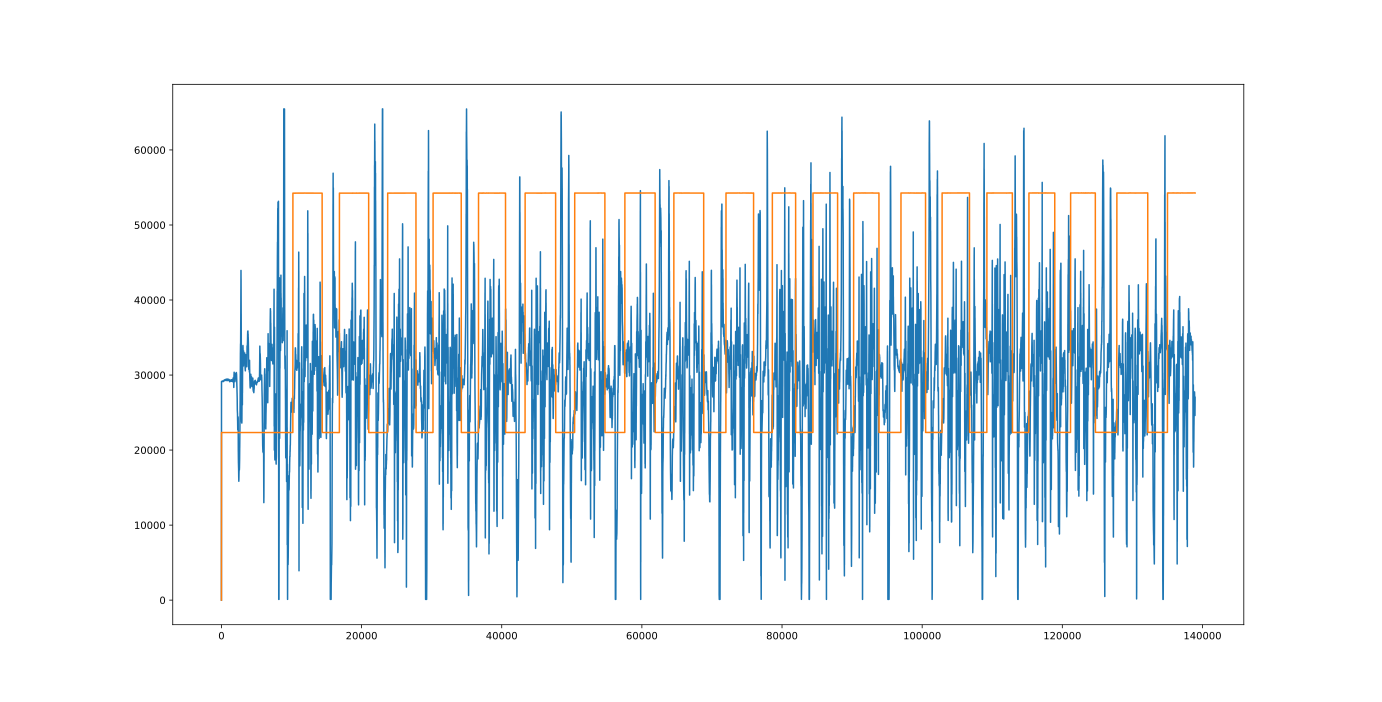
\includegraphics[width=\linewidth]{cyclic_segmentation_example.pdf}
\caption{Segmentation of a walking pattern on a 1D signal with the similarity function ($s_f$). The window size was 5000 samples and the overlap percentage of 75\%.}
\label{fig:cyclic_example}
\end{figure}

Even though the signal is confusing, the method is still able to find the periodic nature. Further, we will show that the method is also robust in more complex datasets, such as with signals from the occupational domain. These signals can have more complex periodic subsequences, where even some motion variety exists from cycle to cycle.

\section{Pattern Search with SSTS}

In order to show the value of using a symbolic representation of the time series and search with regular expressions on that representation, we provide six examples of how to use \gls{ssts} for pattern search on time series and compare the text complexity between the python implementation and the query used, with Halstead measures. 

\subsection{SSTS on selected Use-Cases}

We will present six examples (three more detailed): the second and third examples consist of simple problems that require the detection of local maxima and minima. The sixth example is a more challenging task, which requires the use of more sophisticated mechanisms of the regular expression module. The examples are listed as follows(\textit{Example 1} is omitted since it was discussed in the previous section):\\

\begin{itemize}
\item Example 2 - Step Detection: Detect the instants in time when a right or left heel floor contact is achieved during a normal straight walk from the magnitude of an accelerometer signal. This information can be used to create a step detector based on accelerometer data. Since the sensor is located on the right pocket, global minima will indicate the right heel contact and local minima will correspond to left heel contact;\\

\begin{table}[h]
\centering
\begin{tabular}{ccc}
\toprule
\textbf{Pre-Processing} & \textbf{Connotation} & \textbf{Search} \\
\midrule
LP 2 Sm 50 & A 0.4 D1 0.05 & 0z0p \\
LP 2 Sm 50 &  A 0.3 D1 0.05 & 1z1p \\
\bottomrule
\end{tabular}
\end{table}

\item Example 3 - Segmentation of the systole of the \gls{abp} wave: The dicrotic notch corresponds to the physiological event of the aortic valve closure, which triggers the increase of the aortic pressure and signifies the end of the systolic phase. In this problem, it is asked to segment the systolic phase of the \gls{abp} wave;\\

\begin{table}[h]
\centering
\begin{tabular}{ccc}
\toprule
\textbf{Pre-Processing} & \textbf{Connotation} & \textbf{Search} \\
\midrule
BP 1 20 & A 0.3 D1 0.01 &  (1p).+?0 \\
\bottomrule
\end{tabular}
\end{table}

\item Example 4 - Electrocardiogram peak detector: Detect all the major peaks from an \gls{ecg} record;\\

\begin{table}[h]
\centering
\begin{tabular}{ccc}
\toprule
\textbf{Pre-Processing} & \textbf{Connotation} & \textbf{Search} \\
\midrule
BP 5  50 & D1 0.01 & pn\\
\bottomrule
\end{tabular}
\end{table}

\item Example 5 - Straight Line Trajectory Tracking: The automatic detection of trajectory features, such as straight walks and turns can be used to evaluate trajectory anomalies from a vector of cartesian coordinates in 2D-space;\\

\begin{table}[h]
\centering
\begin{tabular}{ccc}
\toprule
\textbf{Pre-Processing} & \textbf{Connotation} & \textbf{Search} \\
\midrule
none & D2 0.05 & z*? \\
\bottomrule
\end{tabular}
\end{table}

\item Example 6 - Since the first 5 s of the lifting exercise are unstable, the problem involves detecting the first stable lifting step, which occurs approximately 5 s after the beginning of the exercise from an accelerometer signal.\\

\begin{table}[h]
\centering
\begin{tabular}{ccc}
\toprule
\textbf{Pre-Processing} & \textbf{Connotation} & \textbf{Search} \\
\midrule
Mag Abs Sm 1000 {\large \textbf{|}} Mag Sm 750  & A 0.2 {\large \textbf{|}} A -0.2 D1 0.01 & (?<=1.{15000,})(n.p)(.*?)(n.p) \\
\bottomrule
\end{tabular}
\end{table}

\end{itemize}

For the sake of brevity, only three of the examples are presented.

\subsubsection{Use-Case 2 - Step Detection in accelerometer signals}

In this particular case, only the detection of the right heel contact will be discussed, whereas the left heel contact example's solution is presented in Table \ref{tab:Summary}.

\begin{figure}[H]
  \centering
      \includegraphics[width=\textwidth]{ssts_example2.pdf}
  \caption{Example 2 - Solution pipeline of Step Detection example. At the bottom of the figure are summarized the operators and methods used in each step. In the symbolic connotation step, the alternation between the methods is made with colors (Blue - A - Amplitude Comparison, Red - D1 - First Derivative). A dotted line is shown to represent the threshold level. Each color band in the signal corresponds to a specific primitive. A positive match is highlighted with green in the search step.}
  \label{fig:Exercise2}
\end{figure}

The signal is initially pre-processed to ease the identification of the subject's steps. This is achieved using a low pass filter (LP). The result is presented in the second image of the first step in Fig. \ref{fig:Exercise2}. A highlight is also present and delineates a segment of the signal that has a minimum peak, which corresponds to right heel contact. The string representation of this segment is depicted in the second step.
\par
The string is a sequence of primitives composed of two connotation methods (A in blue, D1 in red). Based on these methods, the samples of the signal with amplitudes greater than \textit{40}\% of the range amplitude are transcribed into $1$, while the remaining turn into $0$; the slopes are converted into $p$, $z$ and $n$, when rising, being stationary and falling, respectively.
\par
The solution involves detecting each minimum with an amplitude inferior to the threshold level. The morphological representation of a minimum can be reduced to a negative slope followed by a positive one, which in the symbolic representation is defined by the second connotation method as the transition from $n$ to $p$ or $z$ to $p$. Regarding the amplitude requirement, it is assigned by the first connotation method, in which any value lower than the threshold level is $0$. The regular expression used to find this minimum was $0z0p$, which implies that: (1) the amplitude has to be $0$; and (2) the derivative is $z$ and then $p$. The detection is highlighted in green in the last plot of Fig. \ref{fig:Exercise2}.

\subsubsection{Use-Case 3 - Dicrotic notch detection in ABP signals}

The \gls{abp} waves are morphologically represented by a high positive slope that corresponds to the systolic uptake and ends at the peak of the systolic pressure. After this behavior, follows the systolic decline, which ends with the aortic valve closure, named the \textit{dicrotic notch} in the signal representation~\cite{abpSignal}.
\par
These types of signals are commonly affected by low-frequency noise that modulates the signal and is contaminated with high-frequency noise of low amplitude. The typical procedure is to bandpass the \gls{abp} signal to remove both types of noise. Fig. \ref{fig:Exercise3} depicts how a band pass filter that cuts frequencies under 1 Hz and above 20 Hz (BP) is applied to the signal to remove both types of noise. The modulation removal is shown with the linear regression in both original and pre-processed signals, which in the first case has a positive slope and after the pre-processing is approximately zero.

\begin{figure}
  \centering
      \includegraphics[width=\textwidth]{ssts_example3.pdf}
  \caption{Example 3 - Solution pipeline of Dicrotic notch detection example. The operators or methods used in each step are summarized at the bottom of the figure. In the symbolic connotation step, the alternation between methods is represented with colors (Blue - AD, Red - D1). For each color band in the signal, there is a corresponding primitive. The match is highlighted with green in the search step.}
  \label{fig:Exercise3}
\end{figure}

In the symbolic connotation step, the reasoning follows the signal morphological description and uses two methods for the symbolic representation. The first, AD (represented in blue), detects all rising and falling slopes that are higher than a specific threshold (in this case 30\% of the amplitude range of the signal) and transcribes the sample values to $1$, while the remaining values are converted to $0$. The second method (represented in red) uses the derivative, as mentioned in the previous examples.
\par
The first connotation method is necessary to distinguish between the rising slope that occurs at the beginning of the pressure wave and the one after the \textit{dicrotic notch}. With this distinction, it is possible to find the beginning of the \gls{abp} wave as a high positive slope ($1p$) and find the \textit{dicrotic notch} when the lower slope starts ($0.$). In order to find this area of the \gls{abp} wave, the regular expression has to start with the first $1p$ primitive and end with the first $0.$ primitive. 

\par
The example is solved with the following regular expression: $(1p).*?(0.)$. This string means that the search will match anything (represented by "$.*?$") between the first "$1p$" primitive and the first "\textit{0.}" primitive.

\subsubsection{Use-Case 6 - Stable lifting detection in accelerometer signals}

In the previous example, the solution was achieved by searching for one simple transition in the string generated by the sequence of connotation methods. This tool may also be used to solve more complex examples in the same manner.
\par
The next problem involves the segmentation of a lifting step that has occurred 5 seconds after the start of a weight lifting exercise. The example can be solved in two steps: (1) find the start of the exercise, and (2) search for the segment 5s after the start. This rationale can be expressed by combining two distinct symbolic representations of the same original signal, which requires the use of two pre-processing and symbolic connotation sets, in which one is used for the detection of the start and the other to find the desired segment.

\begin{figure}
  \centering
      \includegraphics[width=\textwidth]{ssts_example6.pdf}
  \caption{Example 6 - Solution pipeline of Stable Lifting Detection. The operators or methods used in each step are summarized at the bottom of the figure. In the symbolic connotation step, the alternation between the methods is made with colors (Blue - AD, Red - D1). The threshold level is identified with a white dotted line. Each color band in the signal corresponds to a specific primitive. The match is highlighted with green in the "Search" step.}
  \label{fig:Hard}
\end{figure}

Fig. \ref{fig:Hard} demonstrates how the example is solved. In both pre-processing and symbolic connotation steps, a vertical bar $|$ separates the methods that are applied for each representation of the same signal. The pre-processing phase uses a sequence of whitening, modulus, and smoothing of the signal for "\textit{Process A}", and a sequence of whitening and smoothing for "\textit{Process B}". The first processing sequence turns the signal similar to a plateau, in which the beginning of the activity is easily identified; whereas, in the second sequence, the signal is smoothed such that each lifting step is well defined.
\par
Regarding the symbolic connotation step, the first method AD (represented in blue) turns all sample values of the first signal that are higher than the threshold level into $1$, while the remaining samples are converted to $0$. The second set is applied to the second signal and uses the derivative of the signal D1(represented in red). Both symbolic connotations merge into a sequence of primitives, in which the first element inspects if the exercise has already started ($1.$)  or not ($0.$), and the second infers the sectioning of the lifting steps, that is if the sample of the signal is increasing ($.p$), stationary ($.z$) or decreasing ($.n$).
\par
The regular expression written to solve the example is $(?<=1.\{15000,\})(n1p)(.*?)(n1p$). Decomposing this expression in the two steps of the example results in: (1) $(?<=1.{15000,})$ and (2)$(n1p)(.*?)(n1p)$. In (1), a \textit{lookbehind} operator is used, therefore, the compiler will search ahead of the first match inside the operator, i.e., the search will match the expression "$1.\{15000,\}$" and search ahead of it. This method aims to handle the temporal dependence between events in the string, in which the number $15000$ is calculated by the number of characters that correspond to 5 seconds in the string. This calculation was achieved by multiplying the sampling frequency, the number of connotations in each primitive, and the desired time, in this case: 1000 Hz, 3 connotations, and 5s, respectively.

\subsection{Measure of Expressiveness}

In order to evaluate parameters of expressiveness with \gls{ssts}, we evaluated the legibility and difficulty in generating the solution for the corresponding task. In the programming field, \textit{Halstead} measures are typically used for this purpose. These measures describe the complexity of the script directly from the source code, based in a set of metrics calculated with the number of distinct \gls{oprt} and \gls{oprd}, and the \gls{Toprt} and \gls{Toprd} (recall Section \ref{subsec:complex} from Chapter \ref{cha:theory}.
\par
The complexity evaluation will be performed to compare the script generated by the \textit{classical} approach with the \textit{syntactic} approach. Concerning the \textit{classical} approach, the list of operators and operands are selected from the \textit{operator} module from python ~\citep{oprtPy}, which includes the list of arithmetic, logical, comparison, bitwise, assignment, and special operators; and, the functions that are used in the resolution process will be set as operators and their corresponding arguments as operands. For example, consider this code line written in python:

\begin{equation}
\centering
pks = peakdelta(s, delta=np.percentile(s, 70) - np.percentile(s, 30))
\end{equation}


\begin{itemize}
\item \textit{\textbf{Total List of Operators}}: '\textit{peakdelta}', '\textit{percentile}', '$-$' and '\textit{percentile}'
\item \textit{\textbf{Total List of Operands}}: '\textit{s}', '\textit{delta=np.percentile(s, 70) - np.percentile(s, 30)}', '\textit{s}', '\textit{70}', '\textit{s}', '\textit{np.percentile(s,30)}', '\textit{np.percentile(s,70)}' and '\textit{30}'
\item \textit{\textbf{List of Distinct Operators}}: '\textit{peakdelta}', '\textit{percentile}' and '$-$'
\item \textit{\textbf{List of Distinct Operands}}: '\textit{s}', '\textit{delta=np.percentile(s, 70) - np.percentile(s, 30)}', '\textit{np.percentile(s, 70)}', '\textit{np.percentile(s, 30)}',  '\textit{70}' and '\textit{30}'
\end{itemize}

In the second case, both \textbf{connotation} step and \textbf{search} procedure will be inspected for the \textbf{difficulty} measures. Regarding the \textbf{connotation} step, the evaluation will be made similarly to the previous method for inspecting functions, in which the function is set as an operator and its corresponding arguments as operands. For the \textbf{search} procedure, the set of instructions typically used in regular expressions (except the "." character) is defined as operators\citep{regex}. These can be revisited in the second section. The remaining characters of the regular expression string, except the parenthesis, will be set as operands. In this are included the "." operator that matches any character, and the "\textbackslash d" and "\textbackslash w" that matches all digits and alphabetical characters respectively. Regarding the parenthesis, when occurring ("\{\}" or "[]"), will be set as one operator. For example:\\

{\centering
\textbf{$Connotation: $} $Sm$ 500  $A$ 0.8 $D1$ 0.05\\
\textbf{$Search: $} \textit{(z1n).*?}\\ }

\begin{itemize}
\item \textit{\textbf{Total List of Operators}}: '$Sm$', '$A$', '$D1$', '( )' and '\textit{*?}'
\item \textit{\textbf{Total List of Operands}}: '\textit{500}', '\textit{0.8}', '\textit{0.05}', '\textit{z}', '\textit{1}', '\textit{n}' and '\textit{.}'
\item \textit{\textbf{List of Distinct Operators}}: '$Sm$', '$A$', '$D1$', '( )' and '\textit{*?}'
\item \textit{\textbf{List of Distinct Operands}}: '\textit{500}', '\textit{0.8}', '\textit{0.05}', '\textit{z}', '\textit{1}', '\textit{n}' and '\textit{.}'
\end{itemize}


\begin{adjustbox}{center, caption={Evaluation of the complexity in the resolution of examples with the \textit{syntactic} approach and with the \textit{classical} approach. Voc - Vocabulary, Lgth - Length, CL - Calculated Length, V - volume, D - difficulty, E - effort.}, float={table}[h!]}
    \small
    \setlength{\tabcolsep}{2pt}
    \renewcommand{\arraystretch}{0.8}
    \label{tab:halstead}
    \begin{tabular}{cl cccccc cccccc}
    	
        \toprule[0.5mm]\\
        
        \multirow{2}{*}{Example} & & \multicolumn{6}{c}{Syntactic Resolution} & \multicolumn{6}{c}{Classical Resolution}\\
        
        \cmidrule[0.2mm](lr){3-8} \cmidrule[0.2mm](lr){9-14} & & \textit{\textbf{Voc}} & \textit{\textbf{Lgth}} & \textit{\textbf{CL}} & \textit{\textbf{V}} & \textit{\textbf{D}} & \textit{\textbf{E}} &
        \textit{\textbf{Voc}} & \textit{\textbf{Lgth}} & \textit{\textbf{CL}} & \textit{\textbf{V}} & \textit{\textbf{D}} & \textit{\textbf{E}} \\      
        
        \midrule[0.3mm]\\
        
        Start/End of Plateau & & 7.0 & 7.0 & 13.6 & 19.7 & 2.0 & \large 39.3 & \maxf{12.0} & \maxf{13.0} & \maxf{33.3} & \maxf{46.6} & \maxf{2.5} & \large \maxf{116.5}\\
         
        \midrule[0.3mm]\\
        
        Step Detection (Left \& Right Heel) & & 7.0 & 8.0 & 13.6 & 22.5 & 2.2 & \large 49.4 & \maxf{19.0} & \maxf{22.0} & \maxf{63.6} & \maxf{93.5} &\maxf{ 4.2} & \large \maxf{388.2}\\
        
        \midrule[0.3mm]\\
        
        Systolic Phase Detection & & 8.0 & 8.0 & 16.4 & 24.0 & 2.5 & \large 60.0 & \maxf{21.0} & \maxf{25.0} & \maxf{73.0} & \maxf{109.8} & \maxf{4.7} & \large \maxf{517.7}\\
        
        \midrule[0.3mm]\\
        
        Electrocardiogram Peak Detection & & 4.0 & 4.0 & 4.8 & 8.0 & 1.5 & \large 12.0 & \maxf{9.0} & \maxf{12.0} & \maxf{20.3} & \maxf{38.0} & \maxf{3.0} & \large \maxf{114.0}\\
        
        \midrule[0.3mm]\\
        
        Straight Line Tracking & & 4.0 & 4.0 & 4.0 & 8.0 & 2.0 & \large 16.0 & \maxf{25.0} &\maxf{33.0}& \maxf{93.5} & \maxf{153.2} & \maxf{5.3} & \large \maxf{811.3}\\
        
        \midrule[0.3mm]\\
        
        Stable Lifting Step Detection & & 13.0 & 21.0 & 35.6 & 77.7 & 4.5 & \large 349.7 & \maxf{22.0} & \maxf{23.0} & \maxf{77.3} & \maxf{102.6} & \maxf{5.0} & \large \maxf{512.8}\\

        \bottomrule[0.5mm] \\
        
    \end{tabular}
\end{adjustbox}

Table \ref{tab:halstead} is presented the performance measures in both ways of solving the demonstrated examples. For the evaluation, the pre-processing step was omitted, which means that only the regular expression is used to compute the difficulty measures for the \textit{syntactic} approach, and only the script after the pre-processing steps is used to compute the difficulty measures for the \textit{classical} approach.


\section{Time Series Classification with Hea\reflectbox{R}TS}

This section is evaluated the ability to perform time series classification with the proposed \gls{hearts} method. For this, it has been applied to the \textit{UCR time series classification benchmark} and compared with the traditional 1-nearest neighbor based on the euclidean distance. As was mentioned on Chapter \ref{cha:ssts}, this process can be performed in multiple ways, namely with the combination of a \textit{Baysian} or \gls{svm} classifiers with either a \gls{bow} or a \gls{tfidf} model. These combinations were also compared. With these evaluations, we expect to conclude (1) if this approach of using a linguistic transformation of a time series with high-level words ordered in time of occurrences is possible with significant performances and (2) which is the combination that best fits this approach.
\par
In addition to these experiments, we performed an individual analysis of several use-cases to understand which is the interpretability and readability of the data based on this linguistic translation. This study should tell us if the words extracted are valuable to indicate the \textit{subsequences} of the time series that are relevant to identify it and distinguish it from others. 

\subsection{Classification Performance}

Figure \ref{fig:distribution_dendogram} shows us how vectorized documents can be compared with the cosine distance to distinguish time series. Simply by using part of the \gls{ssts} queries, it is possible to generate \gls{tfidf} weights that are differently distributed based on the words and how these are ordered on a time series document. Of course, the \textit{Trace} dataset used for this example is a simple dataset, with simple dynamics, but still challenging to classify well with the 1-NN \gls{ed} (only 76\% of accuracy). Therefore, to validate the ability of the proposed method to perform time series classification, it was computed on all datasets of the UCR Benchmark and its performance compared with the standard 1-NN \gls{ed}. The process was divided into two stages. First, the parameters to compute \gls{hearts} were optimized on the standard train and test sets from the \textit{pyts} distribution. The optimized performance was compared with the 1-NN \gls{ed} method. Second, we used the optimized method on 10-fold cross-validation and compared the average accuracies with the 1-NN \gls{ed} (the implementation from \textit{pyts} was used to compute the results of the 1-NN \gls{ed} method).
\par
As mentioned on Chapter \ref{cha:ssts}, the method translates the time series into text with \gls{ssts} queries from Table \ref{tab:ssts_queries}. These have pre-processing, connotation, and search steps. For each step, relevant parameters are necessary depending on the queries used. For this experiment, we used as pre-processing a simple smoothing, which requires a \textit{window size} ($w_s$). The derivative connotation steps also required a specific threshold ($thr$). In addition, the \gls{bow} and \gls{tfidf} models can be built with different \textit{n-gram} sizes. These three parameters were optimized with a grid search method over a range of values:

\begin{equation}
\begin{gathered}
w_s \in [1, 10, 25, 50, 100, 250]\\
thr \in [0.001, 0.01, 0.05, 0.1]\\
n-gram \in [1, 2, 3, 4, 5]\\
\end{gathered}
\end{equation}


We performed the classification with several strategies and combinations, namely: \gls{bow} with Baysian Classifier (BoW+NB), \gls{bow} with \gls{svm} (BoW+SVM), \gls{tfidf} with Baysian Classifier (TF-IDF+NB) and \gls{tfidf} with \gls{svm}. The summary of the performance is presented on Figure \ref{fig:cd_diagram}.

\begin{figure}
	\begin{subfigure}{\linewidth}
    	\centering
    	\includegraphics[width=\linewidth]{cd_diagram.pdf}
    	\caption{Critical distance diagram for the methods that rely in a textual representation of the time series (\gls{bow} and \gls{tfidf}) and euclidean distance for the optimized parameter search.}
    \label{fig:cd_diagram1}
    \end{subfigure}
	\begin{subfigure}{\linewidth}
    	\centering
    	\includegraphics[width=\linewidth]{critical_distance_hearts.pdf}
    	\caption{Critical distance diagram for the methods that rely in a textual representation of the time series (\gls{bow} and \gls{tfidf}) and euclidean distance for the 10 fold cross-validation process.}
    \end{subfigure}
    \label{fig:cd_diagram2}
\end{figure}

As can be seen, the strategies that rely on a \gls{svm} classifier are more robust. The \gls{tfidf} turns out to not be reliable when used with the Bayesian Classifier, which was expected since this type of classifier is purely probabilistic, which is why it works better with the \gls{bow}. On the other end, the \gls{tfidf} model works well with \gls{svm} classifiers, being the best method studied. We then compared it in more detail with the 1-NN \gls{ed} classifier, as presented in Figures \ref{fig:cd_diagram1}, \ref{fig:cd_diagram2} and \ref{fig:comparison_1}.

\begin{figure}[h]
    \centering
    \includegraphics[width=0.95\linewidth]{Hearts_results_2.pdf}
    \caption{right) Classification accuracies for the Bag of Synthatic Patterns in comparison with the euclidean distance combined with 1-NN classifier (1-NN ED) with standard train and test; left) with a 10 fold cross validation.}
    \label{fig:comparison_2}
\end{figure}

The average accuracy for the total 107 datasets is 79\% for \gls{hearts} and 71\% for the 1-NN ED. Special cases are highlighted on Figure \ref{fig:comparison_2}.right. These indicate that the proposed method works poorly in problems with a high number of classes (\textit{Phoneme-39, Adiac-37, PigAirwayPressure-52}, etc...), although some exceptions are found, such as in \textit{PigArtPressure}. Both \textit{Haptics} and \textit{InlineSkate} are badly classified in general by state of the art methods. Binary problems that rely in shapes well described with the derivative properties, such as \textit{ShapeletSim}, \textit{BirdChicken}, \textit{BeetleFly} and \textit{Trace}, are typically better classified.
\par
The same conclusions are confirmed on the 10 fold cross-validation (Figure \ref{fig:comparison_2}.left. Surprisingly, the proposed solution with a \gls{tfidf} and \gls{svm} classifier is very consistent with the previous results, even increasing to 80\% the average accuracy for all datasets. What also is surprising is the improvement of the 1-NN \gls{ed} method, which increased its accuracy to 75\% on average. The critical distance for this performance is now less evident (Figure \ref{fig:cd_diagram2}, but the proposed solution is the overall best method. Even when compared to the other methods, it is overall better in most datasets of the benchmark. The only method that competes is the \gls{bow} with an \gls{svm} classifier, which has a very similar performance (upright scheme of Figure \ref{fig:comparison_1}. 

\begin{figure}[h]
    \centering
    \includegraphics[width=0.95\linewidth]{Hearts_results_.pdf}
    \caption{Classification accuracies for all experimented methods versus the accuracies of the \gls{tfidf} method with an \gls{svm} classifier.}
    \label{fig:comparison_1}
\end{figure}

We wanted to answer two main research questions: (1) can we solve time series classification tasks based on its textual representation following traditional \textit{NLP} methods and (2) could we use the words that describe time series as a readable explanation of the data and the differences between classes. Having evidence that the first point is achieved, we will look into the second point.

\subsection{Interpretable Data Outputs}

Besides the fact that this approach is capable of performing well in classification tasks, we expected to go further by providing some feedback from the textual description, helping to understand what differentiates the classes. The \gls{tfidf} model gives weights for each \textit{word} that characterizes the time series. Searching back the \textit{words} on the time series and summing the weights corresponding to these \textit{subsequences}, a shape relevance is made on the time series, where areas of higher interest and that differentiate the time series from others are highlighted. The next Figures (\ref{fig:interpretable1}, \ref{fig:interpretable2} and \ref{fig:interpretable3}) are displayed showing the highlighted areas based on the \gls{tfidf} weights.
%\par
%In addition to using the weights of the \gls{tfidf} model, it is also possible to extract relevant keywords from the textual representation. This task is called "Keyword Extraction" in the text mining domain. We believe that we can profit from this knowledge to make a more interpretable understanding of what characterizes a time series. This extraction was performed with the \textit{Text Ranking} algorithm on the documents generated for each time series.

\begin{figure}[h]
    \centering
    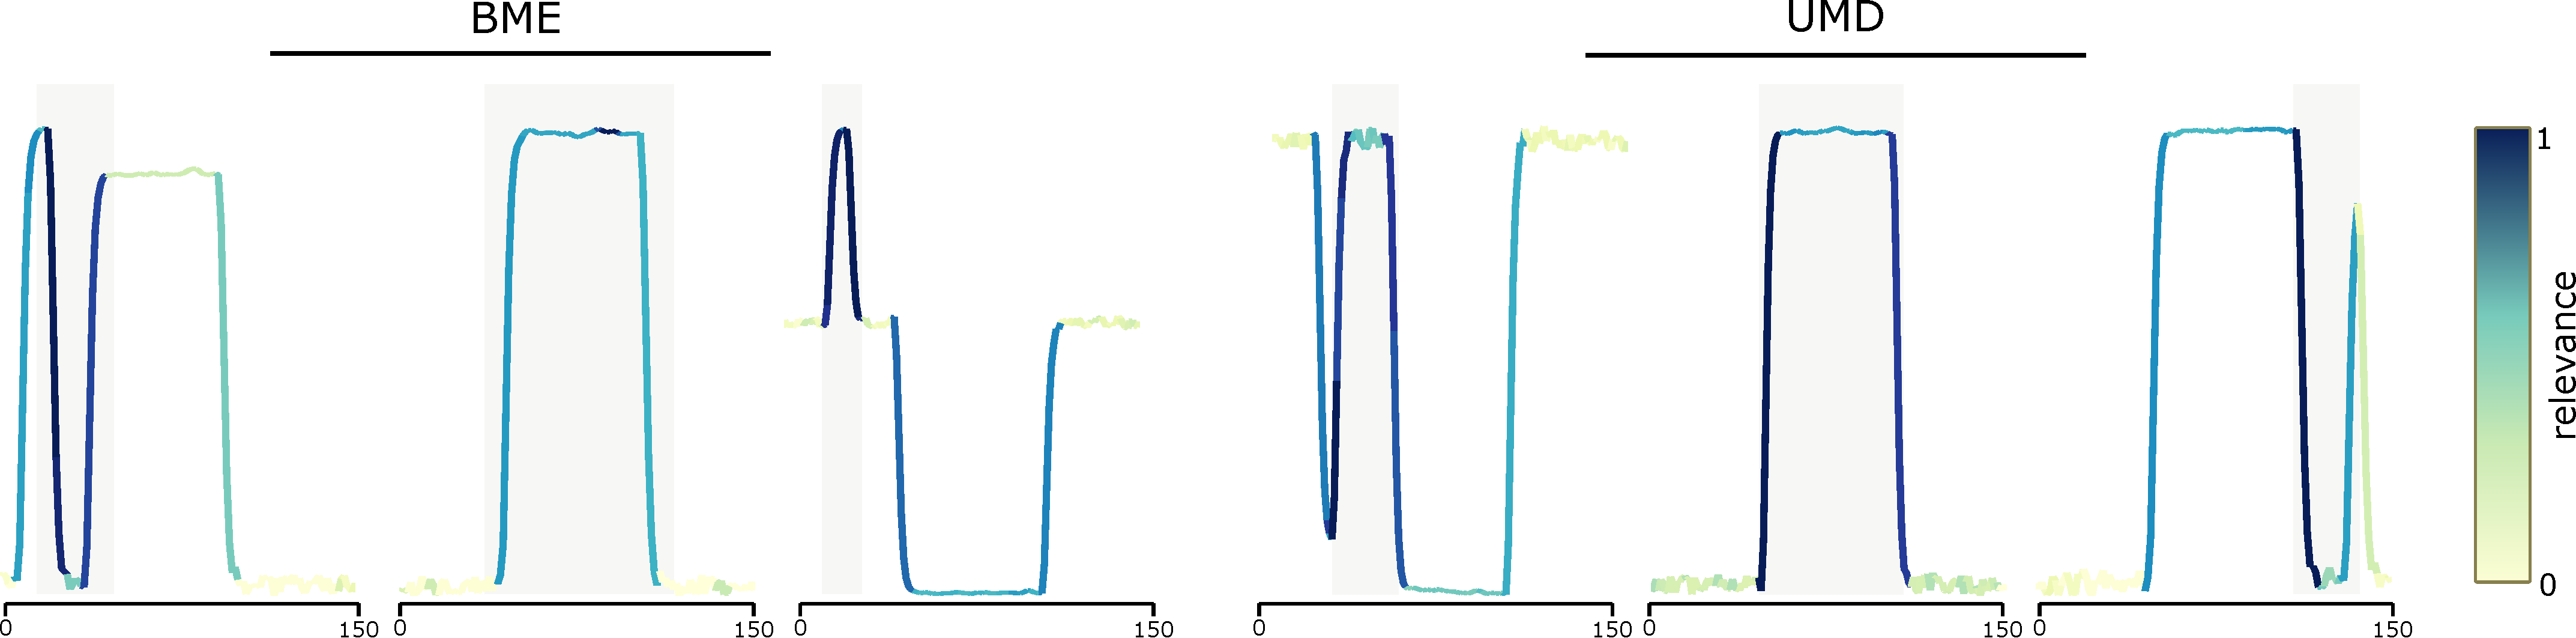
\includegraphics[width=0.95\linewidth]{interpretable_umd_bme.pdf}
    \caption{Interpretable results with highlighted shapes for the \textit{UMD} and \textit{BME} datasets. The \textit{UMD} dataset was classified with with an accuracy of 99.3\%, computed with a $w_s=10$, $thr=0.05$ and a $2-gram$. The \textit{BME} was classified with an accuracy of 100.0\% with a $w_s=10$, $thr=0.05$ and a $2-gram$}
    \label{fig:interpretable1}
\end{figure}

On Figure \ref{fig:interpretable1} are showed two similar datasets. The f1-score of this task was $1$, meaning that it was able to perfectly characterize each shape with the textual representation. For instance, the \textit{BME} dataset has two different sequences of shapes, since the first class has a \texttt{peak followed by a positive plateau}, while the third class has a \texttt{peak followed by a negative plateau}. The second class has simply a \texttt{plateau}. The main difference between all those classes is the peaks and what follows them, which is precisely what is highlighted. The same happens on the \textit{UMD} dataset, in which the most relevant element is the peak and the plateau. As we can see, the transition from the peak to the plateau is highlighted.
%\par
%The keywords extracted are also intuitive. We extracted the top 3 keywords for all samples of time series of each class. For class 1, the following words are the most common: [\texttt{flat}, \texttt{peak}, \texttt{positive plateau}]. For class 2, the most common words are [\texttt{flat}, \texttt{positive plateau}, \textit{high rise}], while for class 3, common words are:[\texttt{fall}, \texttt{peak}, \texttt{high fall}]

\begin{figure}[h]
    \centering
    \includegraphics[width=0.95\linewidth]{interpretable_trace_twopatterns.pdf}
    \caption{Interpretable results with highlighted shapes for the \textit{Trace} and \textit{TwoPatterns} datasets. The \textit{Trace} dataset was classified with with an accuracy of 100.0\%, computed with a $w_s=25$, $thr=0.05$ and a $1-gram$. The \textit{TwoPatterns} was classified with an accuracy of 100.0\% with a $w_s=10$, $thr=0.1$ and a $5-gram$}
    \label{fig:interpretable2}
\end{figure}

Another dataset that is intuitive to understand is the \textit{Trace} dataset. We have been using it frequently in this work and can very easily understand what distinguishes one class from the others. The \textit{subsequences} of interest are highlighted on each time series of each class. For instance, the first class has the \texttt{peak} and \texttt{valley} highlighted, contrasting with the \texttt{valley} from class 2. Classes 3 and 4 have notoriously different valued elements. While class 3 has the rising phase as the relevant shape, class 4 has a \texttt{small peak followed by a valley} on top highlighted.
\par
The \textit{TwoPatterns} dataset is also intuitive to understand and fits the problem for this experiment. Each class has mostly noise, filled with step functions that have different sequences. Class 1 starts by having an \texttt{up} step function and then a \texttt{down} step function. The same logic is applied to the other classes. The proposed method highlights these step functions as being the relevant segments of the signal.

\begin{figure}[h]
    \centering
    \includegraphics[width=0.95\linewidth]{interpretable_gunpoint_shapeletsim.pdf}
    \caption{Interpretable results with highlighted shapes for the \textit{Gunpoint} and \textit{ShapeletSim} datasets. The GunPoint dataset was classified with with an accuracy of 99.0\%, computed with a $w_s=10$, $thr=0.05$ and a $2-gram$. The \textit{ShapeletSim} was classified with an accuracy of 99.4\% with a $w_s=1$, $thr=0.05$ and a $1-gram$}
    \label{fig:interpretable3}
\end{figure}

Finally, two other examples are also presented. One of the \textit{GunPoint} dataset and another from the \textit{ShapeletSim} dataset. The \textit{GunPoint} has 2 classes: (1) the subject draws a plastic gun and points it; (2) the subject simply points with his/her hand. The major difference between the two classes is the drawing process, highlighted by the method as the \texttt{small rise} and \texttt{small fall}.
\par
Regarding the \textit{ShapeletSim} dataset, the data has also two classes. In one, simple shapes, such as triangular, square, or sawtooth waves were added to a random signal. The method can highlight the representative shape of the signal. 

%Some of the most relevant keywords to distinguish it from the other class are: \textit{low Peak}, \textit{high rise} and \textit{high fall}. 

\subsection{Discussion of Results}

In this section, we wanted to answer two main research questions: (1) can we solve time series classification tasks based on their textual representation following traditional \textit{NLP} methods, and (2) could we use the words that describe the time series as a readable explanation of the data and the differences between classes. For this purpose, we applied the proposed method on the \textit{UCR} classification benchmark and highlighted several relevant use-cases and the overall results achieved.
\par
The results provide evidence that it is possible to compare time series based on a textual representation and use traditional strategies from the text mining domain. Not only is it possible to compare the vectors of time series document with the cosine distance (as we have seen on Figure \ref{fig:distribution_dendogram}, but \gls{bow} or \gls{tfidf} models can be used with a linear \gls{svm} to solve classification tasks. The provided results can even be improved considering that the linear \gls{svm} classifier was not optimized.
\par
Additionally, the fact that words are weighted based on their relevance to distinguish each time series document from all the others, it is possible to highlight the \textit{subsequences} of the time series corresponding to these words and understand which parts of the signal are more relevant, being a step forward into interpretability of time series. The limited examples were still simple and intuitive and the process turns harder to understand in more complex data. In these cases, it is hard to truly find meaningful differences and explain why these classes are different, especially with words. This limits the further interpretability potential of this method because the differences might not be perceptible by the naked eye. On one end, the performance can be improved using a richer and correct set of textual descriptors. We mean richer because the differentiation is as good as the description performed, and we mean correct because the translation process from the numerical domain to the text domain is not error-proof, which means that a mistranslation may occur and make the results worse. On the other end, the words used might not be capable of expressing the differences between classes. Many cases with high accuracies can be highlighted, but their interpretability falls short. For instance, for the dataset \textit{BeetleFly}, a binary classification problem. The method has 100\% accuracy but does not show expressively the difference between classes.
\par
The textual representation is valuable in the sense that text mining domain knowledge can be used on time series. Nevertheless, we can profit from this knowledge as much as the translation of the time series into text is rich, valuable, and domain-specific. With the current set of \gls{ssts} queries we can make a limited description that works well in simple signals described mostly by their derivative dynamics. The keywords extracted for these time series still have limited readability being even harder in the complex. However, if more expressive queries are used to make a more robust translation, the keywords extracted can be more valuable and relatable to the time series we are looking at. Therefore, a more diverse set of queries should be used to make possible the extraction of more relevant keywords. At some point, a reduction and selection of the most relevant keywords should be made, as it is performed with feature selection and dimensionality reduction.

\section{Pattern Search with QuoTS}

In this Section, we demonstrate the potential utility of \gls{quots} to search for relevant subsequences in real datasets. Table \ref{tab:operators} from the previous Chapter highlights the keywords and operators if needed to follow these examples. This method, in contrast with \gls{ssts}, uses features and not a symbolic representation of the time series.
\par
In order to show evidence that \gls{quots} is useful in a multitude of scenarios, we present several examples of its application to find relevant patterns on real domain time series. The section will start by presenting how well it matches hand gestures; then show its applicability in searching for relevant patterns in several problems and use-cases; and finally, we present the ability to include additional words based on existing patterns, with the example of \textit{puppeteering} a toy car model.

\subsection{\textit{QuoTS} Matches Gestures}

We start by demonstrating the ability of \gls{quots} to sort how well individual shapes match a written query. For this, we used the \textit{UWaveGestureLibrary} dataset from the \textit{UCRArchive} as a proxy \cite{uWave}, which similar to telemetry data, relies on inertial time series. We use this proxy data simply because it is much larger than any publicly available labeled transportation data. However, we note that gestural interaction with the automobile interfaces is an area of active research \cite{autoui1, autoui2}. With this example, we show that the system can recognize different gestures with or without intuitive queries, hence, if humans were able to learn and master this tool, this recognition problem would be largely solved.

\begin{figure}
\centering
\includegraphics[width=\linewidth]{quots_wavegestures.pdf}
\caption{\textit{UWaveGestureLibrary} subsequence matches with \gls{quots}. Column-wise are showed the gesture class, the corresponding mean wave for all subsequences, the query used to match the subsequence class and the corresponding match score for all subsequences, highlighting with the color of the specific class.}
\label{fig:quots_uwave}
\end{figure}

We not only demonstrate that the system can significantly distinguish gesture patterns, but it does so with very simple and intuitive queries. The ability of the written queries to match the correct class is presented both visually (Figure \ref{fig:quots_uwave} and quantitatively (Table \ref{tab:quots_exp1}). In Figure 5, the set of eight gestures is described row-wise, having a corresponding mean shape (\textbf{MeanWave}) and a query (\textbf{Query}) that should filter it. The visual intuition is demonstrated with the barplot (\textbf{MatchScore}), which for the sake of readability, highlights the normalized match score ([0-1]) of subsequences belonging to the row-wise specific gesture. The other classes are shown in gray. For each gesture, we show the shape of all the available axis (X, Y, and Z). We attempt to create queries using only a single axis (X-axis) but used other dimensions when needed.
\par
To quantify these results, we looked at the top-10 and top-100 matches for each class and counted how many gestures of the selected class were correctly sorted (TP/10 and TP/100). The results are presented in Table \ref{tab:quots_exp1}. These show that the top 10 matches always correspond to the correct class. The reader might think that the first 10 matches might be too easy considering a problem that has around 400 gesture samples per class, but note that having more gesture samples also means more opportunities to make mistakes. Moreover, considering the analogy of searching for a webpage with the \textit{Google} search engine, a user will probably be interested in examining at least the top 10 results. Nevertheless, the reader will appreciate that even if we consider the top 100 matches, \gls{quots} still achieved impressive results.

\begin{table}
\centering
\begin{tabular}{ccccccccc}
\toprule[1.5pt]
& G1 & G2 & G3 & G4 & G5 & G6 & G7 & G8\\
\midrule
TP/10 & 10 & 10 & 10 & 10 & 10 & 10 & 10 & 10\\
TP/100 & 96 & 100 & 94 & 95 & 74 & 100 & 100 & 99\\
\bottomrule[1.5pt]
\end{tabular}
\caption{Results for the top 10 and top 100 sorted gestures classes  (G) when using the queries from Figure \ref{fig:quots_uwave}.}
\label{tab:quots_exp1}
\end{table}

Although we simply wanted to demonstrate that with a set of meaningful words we can correctly sort each of the classes of this dataset, we also want to highlight that the nature of the classes can be very well expressed by the queries. This is especially evident when we look at the query for gestures that are inverse to each other, such as gestures 7 and 8. Gesture 7 is well matched by the query \texttt{[valley peak]}, implicitly, the transposed gesture should have the exact opposite query, which it indeed does (\texttt{[peak valley]}). This also occurs for the two other sets of gestures that occur in natural pair; gestures 3 (\texttt{[bottom up up top] simple}) - 4 (\texttt{[top down down bottom] simple}) and gestures  5 (\texttt{[top down down bottom]}) - 6 (\texttt{[bottom up up top]}).
We also demonstrate that for the handful of cases where this did not work, there was a semantic explanation for it. (e.g. Classes 5 and 6 have not a specific pattern and seem to be especially random in their X-axis, or classes 1 and 2 are very similar, and because of that, are mislabeled). But, as our tool can perform queries in multidimensional data, we can still discriminate these by using the Y-axis in conjunction with X-axis to sort them correctly. 
Note that discriminating among these eight classes is not a trivial problem. Of the more than 1,000 papers to have worked with this dataset, the current best accuracy was obtained by \textit{COTE} algorithm which achieved 76.56\% using a single axis. In addition, this dataset was acquired from eight different subjects, which indicates that our system can account for the intra-subject and inter-subject variability in motion for this dataset \cite{uWave}.

\subsection{\textit{QuoTS} in Selected Use Cases}

In this section, we present several examples of where \gls{quots} can be used in continuous real data. We start with an \gls{ecg} signal that has motion artifacts.

\begin{figure}
\includegraphics[width=\linewidth]{Quots_ecg.pdf}
\caption{\gls{ecg} use case to identify noisy sections, as well as specific segments of the \gls{ecg} pattern. The queries are written in text boxes. On the side, an example of a match is showed as a larger pattern.}
\label{fig:use_case1}
\end{figure}

As a start, we were searching for the motion artifact segment that appears in two areas of the signal. This artifact can be detected in two ways, as we are showing in Figure \ref{fig:use_case1}. The first would be to use the keyword \texttt{noise}, which searches for parts of the signal that have a higher difference from a moving average of the signal. In this case, the higher difference occurs when the motion artifacts appear. We could also search for each of these motion artifact sequences simply by pure visual intuition of their shape. For instance, the first motion artifact looks like a \texttt{valley}, while the second looks like a \texttt{peak}, which ends up matching the desired segments. This process was made by looking for subsequences with 250 samples.
\par
On the \gls{ecg} signal there are also other segments of interest, namely from the \textit{PQRS} complex. In this case, we searched for the \textit{R} \texttt{peak}, the \textit{S} \texttt{valley} and the \textit{T} \texttt{peak}. The first subsequence was simply matched by searching for the keyword \texttt{peak}, with a window size of 50 samples, which contrasts with the 250 samples from the previous example. The keyword matched well the highest peak, but other peaks were present with lower amplitudes, such as the \textit{T} \texttt{peak}. This one was matched with the query \texttt{low peak}. In between these two subsequences, there is the \textit{S} \texttt{valley}. In this case, we show the usage of the special \texttt{followed by} operator. The query \texttt{[high low] [down up]} indicates that the first half of the searched subsequence should have a \textit{high change in amplitude going down} and end with a \textit{low change in amplitude going up}. This is exactly what is matched, as highlighted and indicated by the corresponding \textit{score} function. To be clear, the colored highlighted segments represent the 10-most relevant matches for the written query. The \textit{scoring} functions show that the other matches would be found as well.
\par
The \gls{ecg} signal is a perfect example of how a text-based search can help find relevant occurrences, as there are specific medical conditions that are represented by variations in the original shape of the \gls{ecg} signal. The next Figure (\ref{fig:use_case2}) shows several examples of the detection of three different types of arrhythmia from the \textit{St Petersburg INCART 12-lead Arrhythmia Database} (Physionet) \cite{PhysioNet}.

\begin{figure}
\includegraphics[width=\linewidth]{Quots_ecg2.pdf}
\caption{Examples of the detection of three specific cases of arrhythmia. The ground truth is selected from the annotations of specialists in the area. The queries are presented in text boxes and the found patterns are highlighted. On the side, an example of a match in a larger size is shown.}
\label{fig:use_case2}
\end{figure}

The ground truth follows the annotations present on the original files. Three types of annotations were found, associated with different types of arrhythmia events (A - \includegraphics[height=2.5ex, valign=m]{arrhytmia_A.pdf}, F - \includegraphics[height=2.5ex, valign=m]{arrhytmia_F.pdf} and V - \includegraphics[height=2.5ex, valign=m]{arrhytmia_V.pdf}). Using \gls{quots}, we can search for these occurrences in the presented segment. The first event is characterized by having a normal beat irregularly before it was supposed to. It is then possible to find two \gls{ecg} beats in a shorter window. This means that if we search for two main peaks inside a short window, separated by anything (\texttt{.}) \texttt{III: [. peak . peak .]} (in this case 500 samples on the lead III), it should be possible to find where these events occur. We displayed the 5-top subsequences that match the query and the corresponding scoring function. Four out of the five events are highlighted, but the scoring function indicates that the "missing" subsequence has a high match value as well. The wrongly identified event fits the description as well, being a different type of arrhythmia, but with a different shape (type F). This shape is normally a high change in amplitude, therefore if we state that we reject any high amplitude change subsequence, we should be able to match the five desired subsequences. Adding \texttt{!high} to the previous query (\texttt{III: [. peak . peak .] !high}) leads to correctly matching all the desired subsequences. To be clear, we chose lead III without any specific purpose, being possible to use the other leads for the same purpose. What matters is that the desired subsequence has a particular characteristic that differentiates it from the rest.
\par
The second example corresponds to the arrhythmia of type F, characterized by a high change in the amplitude of the \gls{ecg} with an irregular beat. In this case, we can match this event with the simple query \texttt{AVL: [high peak]}. Other events are matched but have a much lower amplitude. The other events matched are from the type V, which does not present a long flat section after the irregular beat. In this case, the lead AVR shows a very specific difference from the other two types of arrhythmia, which is the fact that the beat occurs on top, deviating from the middle of the signal. The shape continues to be a \texttt{valley} but on \texttt{top} (\texttt{AVR: valley top}). It is relevant to point out that the original annotations (ground truth) do not include one of the highlighted subsequences. Although not confirmed with a specialist, the shape of the event in all \gls{ecg} leads are the same for this type of arrhythmia, so we suspect that there was a missing label that the query was able to indicate.
\par
In addition to searching for specific shapes on signals, \gls{quots} can be very useful for exploratory purposes in multivariate datasets. For instance, consider the following examples on a dataset acquired with the purpose to identify workload on drivers \cite{hci_car_dataset}. In this experiment, drivers physiological signals, such as \gls{ecg} and \gls{scr}, were monitored. Exploring this dataset with \gls{quots} led to discovering several interesting occurrences, as shown in Figure \ref{fig:quots_car_physio}. In this Figure are signaled specific events with road signs. We matched these signs' positions by finding their \textit{latitude} and \textit{longitude} on the map and matching them with the instant in time these coordinates occur on the dataset. In addition to this information, we recall the common terms used for auto telemetry, namely: Surge - breaking (peak) and accelerating (valley); and Sway - turning right (peak) or left (valley).

\begin{figure}[h]
\centering
\includegraphics[width=0.85\linewidth]{quots_car_bio.pdf}
\caption{Example of multivariate patterns on a dataset from auto telemetry with physiological signals of the driver. The queries are written in text boxes. Several matches are highlighted based on the queries written. These events are associated with specific occurrences during the driving session, symbolized by traffic signs. These events were matched by searching the coordinates on the map. \cite{hcilab}}
\label{fig:quots_car_physio}
\end{figure}

The first found events were identified by searching for moments where the driver was pulling the breaks and at a similar moment in time, the driver was having an increasing value of skin conductance (indicative of higher sweat and possibly momentary stress). The query can be written as \texttt{Surge: peak high SCR: up}. We found that the presence of such events is very high on two occasions, in both cases, right before a traffic light. The second traffic light was turned red because the car stopped. This led to searching for a moment where the driver started accelerating and the skin conductance was increasing (\texttt{Surge: valley SCR: up}), which points to two main locations on the signal. The second is exactly when the car started driving after stopping at the traffic light, suggesting to be a relevant reaction from the driver. We did not have access to the videos, and can only guess what happened during the driving experience, but we can conclude that these identified moments are relevant to be observed afterward on the video, highlighting that \gls{quots} can be used to explore the signals very quickly, identify moments of interest (especially correlating multivariate variables) and search them on the video to validate what happened. 
\par
In addition to these events, we searched for moments where the driver had to break and then turned. There is a time dependency between these two occurrences and can use the \texttt{followed by} operator for this purpose. Therefore, we searched for \texttt{Surge: peak high followed by Sway: high}. The results pointed out several locations on the signal, three of them associated with turning right at a crossing and two roundabouts.

\subsection{Matching \textit{Known} Shapes with Words}

We believe that \gls{quots} can be developed to be intuitive enough to allow most novice users to create simple effective queries for most information retrieval tasks.  However, in some cases, the user’s ability to formulate queries may be a limitation. In this section, we show that it is possible to perform a \textit{mimicry} of the process being searched and add the query designed with the mimicry process as a \textit{word feature vector} inside our vocabulary. We show a few examples of possible applications, starting with "puppeteering" a model car in performing a 3-point-turn. First, we will show the signal where we searched this event and how we used \gls{quots} to find it with a text query.

\begin{figure}
\includegraphics[width=\linewidth]{quots_3pointturn2.pdf}
\caption{Example of searching for a 3 point turn event with \gls{quots}.}
\label{fig:quots_3pointturn}
\end{figure}

Figure \ref{fig:quots_3pointturn} is showed the search for a 3-point turn on a signal acquired with a smartphone inside a car while performing several driving exercises in a parking lot. Details of the experiment can be found at \cite{quots_github}. The query used to match this event is very intuitive, being \texttt{[peak peak peak]}, which is exactly what this pattern is (\includegraphics[height=2.5ex, valign=m]{3pointturn.pdf}). 
\par
Having found the desired pattern with text, we thought that it would also be possible to find it using a specific pattern and give it a name, to use on \gls{quots}. In this case, the pattern was acquired with a toy model car, on which a smartphone was attached (as indicated in Figure \ref{fig:puppeteering}) and acquired inertial data while mimicking a 3-point turn event on a table. The resulting shape is illustrated in \textit{puppet data}. We believe this can be used in two ways: for the user to gain intuition as to how a motion/\textit{manoeuver} is illustrated on motion data or how the inertial data from the motion/manoeuver can be used as a template on \gls{quots}: \\
•	\textbf{Shape Intuition:} A user might not know what the shape of a 3-point turn looks like. By using a model car, he/she can mimic the motion and gain intuition over what the query should be (in this case, \texttt{[peak peak peak]}). \\
•	\textbf{MASS template:} As mentioned above, we have a special shape word, which corresponds to a shape template given by the user, to which a word can be assigned. We then can use the word in our language to match desired patterns with the MASS distance profile as a word feature vector.  

\begin{figure}[h]
    \centering
    \includegraphics[width=0.95\linewidth]{toycar_puppet_example.pdf}
    \caption{Creating query prompt data by puppeteering a car model. The puppet data for a 3-point turn (smoothed with 10 samples moving average) is presented on the left, while the real data from a real car is presented on the right. }
    \label{fig:puppeteering}
\end{figure}

We added the puppet data and the word \texttt{3pointturn} to our vocabulary. Searching for it in the signal matched all the desired shapes. Note that the template has a different amplitude and time scale considering that the motion was made with our hand, but the z-normalization makes the amplitude difference irrelevant, and the time scale was adjusted by resampling the template based on the selected window size for the query search. With this, the template is not only a template, it also becomes part of the language, being used in combination with all the other words available in our vocabulary.


\section{Application to Occupational Scenario}
\label{cha:application_occ}

%In occupational settings of the \textit{Volkswagen} Autoreuropa plant, workers mostly perform repetitive and cyclic tasks during their working day. These cyclic tasks are sometimes interrupted by stoppages on the assembly line due to delays in other areas, breaks by the worker, or even the case where the work shifts to another workstation to help a colleague or take over another type of task.
%\par
%When performing occupational data analysis for risk evaluation, the analyst has to differentiate the moments of interest (active working periods) from the rest (nonworking periods). To be clear, the nonworking periods do not mean that the worker was motionless, but only that he/she was not performing the specific repetitive task. In addition, the process of risk analysis is made by working cycle. In that sense, the cyclic information of these cycles has to be segmented as well for the analysis.
%\par
%In this section we show several examples where the \gls{ssm} can be used in this multidimensional information for several tasks in data processing, before the risk analysis.
%
%\subsection{Segmentation 1: Active and Non-Active Periods}
%
%As explained in Section \ref{sec:industry} with Figure \ref{fig:example_industry}, the signal can have several active and non-active periods. The \gls{ssm} was used with the \textit{nova} function to extract the transitions between these sections.
%
%\begin{table}
%\caption{Results of type event 1 (work period transition), discriminated per time serie samples. Measurements of \gls{P}, \gls{R}, \gls{F1}, \gls{A} and \gls{mae}, of each according sample.}
%\label{table:auto_scores}
%\centering
%\begin{tabular}{llllll}
%\toprule
%TS sample         & \gls{P}    & \gls{R} & \gls{F1}    & \gls{A}  & \gls{mae} (s) \\
%\midrule
%Operator 1 Workstation 1      & 0,78 & 1 & 0,88 & 0,78 & 11,87   \\
%Operator 1 Workstation 2      & 1    & 1 & 1    & 1    & 34,77   \\
%Operator 2 Workstation 1\&2 & 0,86 & 1 & 0,92 & 0,86 & 10,17   \\
%Operator 3 Workstation 1    & 0,80 & 1 & 0,89 & 0,80 & 3,21    \\
%Operator 4 Workstation 1    & 1    & 1 & 1    & 1    & 8,83    \\
%Operator 5 Workstation 1      & 1    & 1 & 1    & 1    & 8,54    \\
%Operator 5 Workstation 2      & 1    & 1 & 1    & 1    & 8,38   \\ \hline
%\bottomrule
%\end{tabular}
%\end{table}
%
%The detection of transitions between active to non-active segments was possible with the usage of the \gls{ssm}. In Figure \ref{fig:stortytell}, the reader can notice that there are very clear \textit{block} structures that indicate this change. In addition, as this segment is highly different than the rest of the signal, it has very low values on the similarity function.
%\par
%Having found active periods of work, the next step would be to segment each cycle of the task.
%
%\subsection{Segmentation 2: Working Cycles}
%
%\begin{table}
%\centering
%\caption{Detected cycles and \gls{D_e} results of the detection of type 2 events, over the \textit{Industrial} database.}
%\label{tab:wc_results}
%\begin{tabular}{lcc} 
%\toprule
%\multirow{Signal} & \multicolumn{2}{c}{\textit{\gls{ssm}}}\\
%                                                         & Detected Cycles & Duration Error\\ 
%\midrule
%\gls{Opr}1 \gls{Wkst}1 & 11/11           & 3.26s (3.04\%)  \\
%\gls{Opr}1 \gls{Wkst}2 & 14/15           & 16.97s (15.83\%)\\
%\gls{Opr}2 \gls{Wkst}1 & 14/14           & 6.45s (6.40\%)   \\
%\gls{Opr}2 \gls{Wkst}2 & 11/11           & 8.48s (8.62\%)   \\
%\gls{Opr}3 \gls{Wkst}1 & 16/16           & 12.35s (11.79\%)\\
%\gls{Opr}3 \gls{Wkst}2 & 13/13           & 8.81s (8.25\%)   \\
%\gls{Opr}4 \gls{Wkst}1 & 14/14           & 1.05s (0.4\%)    \\
%\gls{Opr}4 \gls{Wkst}2 & 11/11           & 3.42s (3.32\%)   \\
%\gls{Opr}5 \gls{Wkst}1 & 12/12           & 2.83s (2.85\%)   \\
%\gls{Opr}5 \gls{Wkst}2 & 10/11           & 3.47s (3.45\%)   \\
%\gls{Opr}6 \gls{Wkst}1 & 14/15           & 3.79s (3.74\%)   \\
%\gls{Opr}6 \gls{Wkst}2 & 14/15           & 5.79s (5.73\%)   \\ 
%\midrule
%\multicolumn{1}{c}{Total}                                & 154/157             & 6.12\%\\
%\bottomrule
%\end{tabular}
%\end{table}
%
%From the 157 working cycles, 154 cycles were detected. The duration error was still significant, with a value of 6.12\% of the working cycle. This can be explained based on our justification for Dataset 4, which has a high \gls{mae}. The fact that the window that extracts features is very large, makes the method less precise. Still, it can segment the time series in the same moment of the working cycle.
%\par
%An interesting fact about this data is that some working cycles are not made of one distinctive sequence of motions, but rather a junction of several stages that have similar motions. Being able to segment the entire cycle is, therefore, more difficult and relevant.
%\par
%The proposed method proves also to apply to several scenarios, namely different activities, performed in different workstations, and can manage inter-subject variability.
%
%\subsection{Segmentation 3: Storytelling Data}
%
%As a concluding note, we believe this method support telling the story behind the data. It can help identify moments that are relevant and try to figure out their meaning with minimal context. For instance, taking the example of Figure \ref{fig:autoeuropa_ssm}, a worker was performing workstation 1, was interrupted for a long period, restarted to perform workstation 1, and then shifted to workstation 2. This sequence of events is possible to be seen on the \gls{ssm} of the signals monitored.
%
%
%
%
%
%%For instance, before showing an example of the occupational domain, let us show the reader an example of Dataset 4.
%%
%%\begin{figure}
%%    \centering
%%    \includegraphics[width=\linewidth]{Clustering_real_difficult_timeseries.pdf}
%%    \caption{Activity segmentation and clustering based on the \gls{ssm} for an example of Dataset 4. The activities are color coded, as well as the segments identified by the analysis of the \gls{ssm}. These are then clustered based on the similarity profiles (which are also colorcoded on the dendogram).}
%%    \label{fig:example2_har}
%%\end{figure}
%%
%%Figure \ref{fig:example2_har} shows a signal with several activities (as described in Section \ref{subsec:uci}). The transitions are relatively easy to identify. After segmenting these transitions, we can sort them by their corresponding activity class. Besides, all subsequences related to standing (standing, walking, climbing, or falling stairs) are grouped, while static postures such as sitting or lying are closer together.
%
%\subsection{Storytelling Occupational Data}
%\label{subsec:storytel}
%
%1 - Example of the data we acquired in Volkswagen when we arrived and tried to compare two workstations. We were trying to find specific cyclic moments and labeled them by hand. We can use this tool to make this identification (SSM):
%
%1.1 - show the matrix of the data
%
%2 - Describe the pattern using words or a regular expression
%
%
%%Another example is from an industrial scenario, where a worker performed cyclic activities and was interrupted several times \cite{antonio, santos_explaining_2020}. The novelty function can segment the areas of work versus pause and the similarity function indicates where the working cycles occurred with local minima in the similarity function.
%%
%%\begin{figure}
%%    \centering
%%    \includegraphics[width=0.9\linewidth]{example_industrial.png}
%%    \caption{Example of a worker performing cyclic tasks in an industrial setting. The worker has interruption in his/her work which are annotated with the red labels. The novelty (nova) and similarity (sim) functions are computed from the \gls{SSM} generated with a window size of 2500 samples, overlap of 85\% and kernel size of 50 samples.}
%%    \label{fig:my_label}
%%\end{figure}
%
%\subsection{Pattern Search in Occupational Data}
%\label{subsec:search}
%
%\section{General Limitations}
%
%In this section we present the general limitations of the presented methods, following the results achieved.
%
%\subsection{Information Retrieval with the SSM}
%
%- size and memory consumption
%
%- feature reduction
%
%- feature specific
%
%- The method to retrieve the diagonals is not good enough
%
%- The summarization process is not good enough
%
%- To put it online might be a bit tricky
%
%\subsection{Pattern Search with SSTS}
%
%- requires knowledge of regular expressions
%- should tend to a higher level of legibility, converting sequences of characters into words
%- can still be optimized in search speed with compression methods
%- The search process should be more flexible 
%
%\subsection{Classification with HeaRTS}
%
%- the readability is still limited, with words that come as output not always making sense.
%
%- the method works well with simple shapes that are based on derivative properties
%
%- the classification process is as good as the diversity of words used to describe it, a better vocabulary should be used to have better results and capture the essence of the transitions
%
%\subsection{Pattern Search with QuoTS}
